The design of the implemented quantum computer simulation is based on a library design pattern. As such there is no strict usage of the source code, a host program simply imports the packages it requires. The source code was packaged into discrete packages to enable maximum extensibility. Four main packages are contained in the project: \emph{Core, Core.Math, Operators} and \emph{Algorithms}. The \emph{Core} package contains the fundamental classes required to represent a quantum computer, with the \emph{Core.Math} package containing the mathematical structures required. The \emph{Operators} and \emph{Algorithms} packages are extensions of the \emph{Core} package, which implement common operators and algorithms on quantum computers.

The \emph{Core} package contains a single implementation: \emph{QRegister}, representing a quantum register and three interfaces, \emph{Operator, Algorithm, AlgorithmOutput}. The \emph{Operator} interface is a representation of a linear operator and its interaction with \emph{QRegister} objects. The \emph{Algorithm} interface is defined such that an \emph{Algorithm} has a run method, either classical or quantum. In combination with \emph{Algorithm} we needed a variable output type to be the result of all algorithms, the \emph{AlgorithmOutput} interface represents this in such a way that the only requirement of the output of an algorithm is that it has a human readable string associated with it.

\begin{figure}[H]
	\centering
	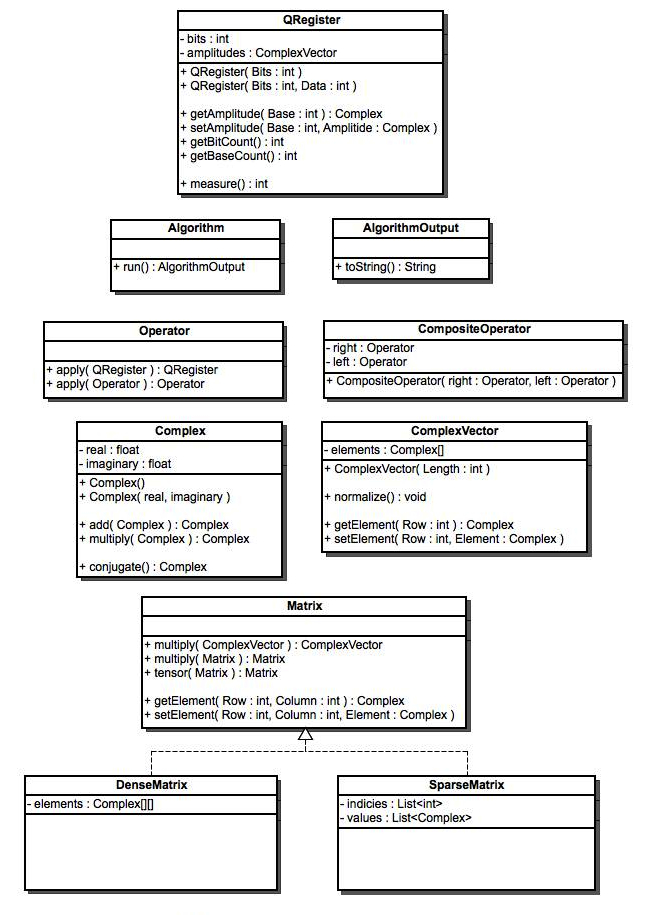
\includegraphics[width=140mm]{./images/design}
	\caption{UML description of the \emph{Core} package and \emph{Core.Math} package.}
\end{figure}